% !TEX root = ../../../main.tex
% 来源：中学数学实验教材·第二册（几何）
% 章节：实验几何 / 基本作图
% 原始文件：1.tex，行 3915-3924
% 类型：tikz
% ---
\begin{tikzpicture}
\tkzDefPoints{0/0/A, 2/0/B, 1.5/1.2/C}
\tkzDrawSegments(A,B A,C)
\tkzDefPoints{4/0/A', 5.5/0/B', 5.5/1.3/C'}
\tkzDrawSegments(A',B' A',C')

\tkzMarkAngles[mark=none, size=.4](B,A,C B',A',C')
\tkzLabelAngle[pos=.6](B,A,C){$\alpha$}
\tkzLabelAngle[pos=.6](B',A',C'){$\beta$}
\end{tikzpicture}
